% !TEX root = ../main.tex

\section{Results}
\textbf{Ignore color coding of concepts for now - we can determine style macros later}
\newline
In our concept dependency graph, use cases depend on capabilities, which are specific high-level functions that blockchain can provide to solve real-world problems. In turn, capabilities are enabled by technological properties, which are provided by specific primitives. See Fig. XX for an example.  The primitive \primitive{hash chain} provides the property \techproperty{append-only transaction ledger}, which in conjunction with other properties enables the capability for \capability{internal auditability}. Use cases in the provenance family require internal auditability to ensure valid provenance trails.
\textbf{TODO: add figure showing graph and text style legend}

We will begin with an overview of the capabilities we generated during selective coding, then discuss results gained by analyzing the construction of the graph and applying some simple heuristic analysis such as identifying nodes with especially high or low degrees of connectivity.

\subsection{Terminology}
TBD

\subsection{Capabilities}
\paragraph{Provenance} These systems track and store records of how assets are created, handled, accessed, and modified. A blockchain can serve three different capabilities by associating \primitive{on-chain tokens} with different types of assets: \capability{physical off-chain asset provenance} (e.g., for real-world objects like diamonds), \capability{digital off-chain asset provenance} (e.g., copyrighted digital media like songs), or \capability{digital on-chain asset provenance} (e.g., Bitcoin), in which the tokens themselves are the asset being tracked. As events happen to an asset (e.g., it is accessed, modified, or it changes ownership), the state of the token is updated accordingly, creating a provenance ledger on the blockchain. For on-chain assets, this correspondence can be ensured, but \primitive{off-chain stapling} is necessary to ensure that events on off-chain assets are properly recorded on the blockchain.

Provenance capabilities all rely on an \techproperty{append-only transaction ledger}, because provenance must be immutable to be useful. The ledger consists of a series of \primitive{transactions}, which are ordered through \primitive{timestamping} and stored in an \primitive{authenticated data structure} (a \primitive{hashchain}, \primitive{hash DAG}, or \primitive{Merkle tree}). 

\paragraph{Smart contracts / automatic code execution} A program stored on a blockchain can be executed automatically in response to function calls added in later transactions. These programs, sometimes called \capability{smart contracts}, can modify the global state of the blockchain (i.e., by moving Ether from one address to another). Miners enforce \techproperty{replication rules} on transactions to determine what types of programs the blockchain supports. This property depends on the \capability{governance} capability, its primitive dependencies \primitive{Sybil resistance} and \primitive{game theory}, and the following additional primitives: \primitive{transactions}, \primitive{authentication}, and \primitive{off-chain oracles}.

\paragraph{Auditability} Blockchain-based systems operate by enforcing \techproperty{replication rules}, which define what state changes are valid. Because the \techproperty{append-only transaction ledger} stores the full history of state changes, it is possible to audit the system to determine what operations occurred and that they were validated. Any blockchain permits \capability{internal auditability}, meaning that validators can perform audits. Blockchains that allow \normproperty{public participation} can further support \capability{public auditability}, meaning that anyone can perform an audit.

\paragraph{Resilience} Broadly speaking, resilience describes the ability of a system to recover from compromises and maintain operation even when in a compromised state. There are three key blockchain capabilities in the resilience family. First, \capability{data replication} mitigates attacks that target data at rest. Second, the properties of Blockchain as a \techproperty{distributed ledger} and an \techproperty{append-only ledger} allow for \capability{verifiable data store rebuilding}. Finally, \techproperty{decentralization} (and particularly {\capability{decentralized governance} and \primitive{peer-to-peer communication}) results in \capability{no single points of failure}, removing obvious targets for attack such as transaction processors or centralized communication servers.

\paragraph{Access control for tokens} This capability permits various data sharing use cases by allowing for access control policies to be enforced using tokens. The primitives that directly support it are: \primitive{PKI}, \primitive{key management}, \primitive{authentication}, and \primitive{on-chain tokens}.

\paragraph{Data discoverability} This capability relies on a \techproperty{distributed data store} to replicate data across many peers, permitting collective maintenance and access to the data. Peers agree on the contents of the store by running a \techproperty{consensus protocol}, which in turn relies on \primitive{peer-to-peer communication} and \primitive{timestamping}. 

\subsection{Graph Analysis Theories}

\paragraph{Decentralized governance is the central capability of Blockchain}
\techproperty{Decentralization} is enabled by \capability{consensus}-based governance, of which Blockchain permits two types: \techproperty{public governance} and \techproperty{permissioned governance}. Either can rely on \primitive{on-chain incentives} (such as Bitcoin block rewards) or \primitive{off-chain incentives} (e.g., contractually obligated payment) to encourage honest behavior from governors. Full decentralization -- i.e., public governance -- further relies on \primitive{Sybil resistance} to prevent individuals from presenting multiple identities to increase their governance share.

This subgraph is central in our dependency graph; it makes use of a large proportion of primitives, is strongly interconnected to other capabilities, and supports many use cases. As such, we interpret the ability to operate a shared system and transact between parties without reliance on any centralized parties as a core feature of Blockchain technology. Many of the use cases in our graph, such as \usecase{payments}, \usecase{identity management}, and \usecase{gambling}, are well-studied problems with obvious or widely known centralized solutions; the primary benefit of developing blockchain-based solutions to these problems is to eliminate centralized processing. Thus, we pose the following question as an initial litmus test for evaluating whether a problem well-suited for applying blockchain: \textit{does it require decentralized governance or operation?} While an answer of "no" does not necessarily mean that Blockchain is not necessary, a "yes" is a very strong indicator that a blockchain may be the right solution.

\paragraph{Anonymity and privacy are orthogonal to the core functions of a blockchain}
Several authors in our corpus cite \capability{anonymity} or privacy as features of Blockchain, although these terms are rarely defined precisely. The main belief seems to be that Blockchain has the property of \techproperty{anonymous transactions} -- i.e., it hides the sender and receiver of asset transfers and disassociates on-chain identities from real-world identities. These notions are connected to Blockchain's reputation for enabling illicit activity (see section~\ref{subsec:challenges} for a discussion of this challenge). The thinking goes that because Bitcoin is the currency of choice for illicit online purchases, it must be "untraceable", and as the most prominent blockchain-based system, distinctions are not drawn between properties of Bitcoin and properties of Blockchain.

Copious literature demonstrating the lack of privacy and anonymity in Bitcoin aside (\cite{Goldfeder17}, \cite{Conti17}, \cite{Androulaki13}, and others), our graph reveals that anonymity is a weakly-connected capability, leveraging few of Blockchain's core primitives and and supporting \textbf{no} use cases. While advanced cryptography like \primitive{multi-party computation}, \primitive{functional encryption}, and \primitive{zero-knowledge proofs} could be layered on top of a blockchain to provide some form of anonymity, only the last primitive appeared in our corpus. \techproperty{Key-based ownership of tokens} is the only property that supports anonymity and also derives from at least one core blockchain primitive (specifically, \primitive{authentication}).

\paragraph{Resilience is a broadly supported capability that is easy to overlook}
As described above, there are three capabilities that provide resilience: \capability{data replication}, \capability{verifiable data store rebuilding}, and \capability{no single points of failure}. These capabilities are supported by key technical properties (\techproperty{distributed data store}, \techproperty{distributed ledger}, and \techproperty{decentralization}), but resilience as a whole is only directly required by a few use cases. This makes the significance of the capability easy to overlook. However, there are a few pieces of important auxiliary information that underscore its importance:

\begin{itemize}
	\item In general, distributed systems aim to be resilient to disruption. This is one of the reasons to distribute a system rather than run it centrally. Because most blockchain applications are distributed systems, we judge that this capability is of high value even though it does not directly enable many use cases. In other words: although there are few Blockchain applications that cannot exist without resilience, there are many that benefit from it.
	\item Resilience is more of a principle than a specific technical capability, and it can only be defined or measured with respect to a specific threat model. The three capabilities that we identify as providing resilience each do it along a different technical vector, protecting against different threats and thus providing a very broad definition of resilience. This too contributes to the high value we ascribe to the capability.
\end{itemize}

\paragraph{Normative and technical properties are cleanly separable}
When reading papers or participating in discussions about Blockchain, it can be difficult to separate normative statements from technical ones (see section~\ref{subsec:challenges} for a discussion of this challenge). In our concept graph, however, technical properties and normative properties cleanly separate. No capabilities have dependencies on normative properties, and removing them from graph does not lessen the value of the graph as an exploration of technical concepts. The injection of ideology into a technical field causes confusion and suboptimal design choices -- not to mention muddying discussion and preventing clarity -- so we believe this surprising result is of value to the field in so far as it may help to resolve these issues.

\paragraph{Blockchain can serve as both a ledger and a data store, but it's better as a ledger}
Two highly-connected, central nodes in our graph are \techproperty{distributed data store} and \techproperty{distributed ledger}. Both rely on a \techproperty{consensus protocol} to ensure consistency across the different data storage locations. The distributed ledger further requires an \techproperty{append-only transaction ledger} to ensure that once consensus has been reached on a transaction, it can no longer be modified. 

As a distributed data store, Blockchain can provide two useful capabilities: \capability{data discovery} and \capability{resilience} (through \techproperty{replication}). As a distributed ledger, Blockchain also provides resilience through \capability{verifiable data store rebuilding} (which allows a node to recover to the current ledger state even if it suffers local data loss). Further, the ledger enables two important groups capabilities that support many use cases: \capability{auditability} and \capability{provenance}. 

This shows that Blockchain's significant novel utility is more firmly rooted in its ability to provide a distributed ledger of state changes than the simple maintenance of a single shared state.

\subsection{Classifying Blockchain \bnote{In Progress}}

Our grounded theory analysis revealed that the key properties of a blockchain are decentralized governance, auditability, and resilience. To understand how Blockchain relates to other types of data stores, we organized these properties into a series of classifying questions. Figure~\ref{fig:blockchainFlowchart} shows the results.

\begin{figure*}
	\centering
	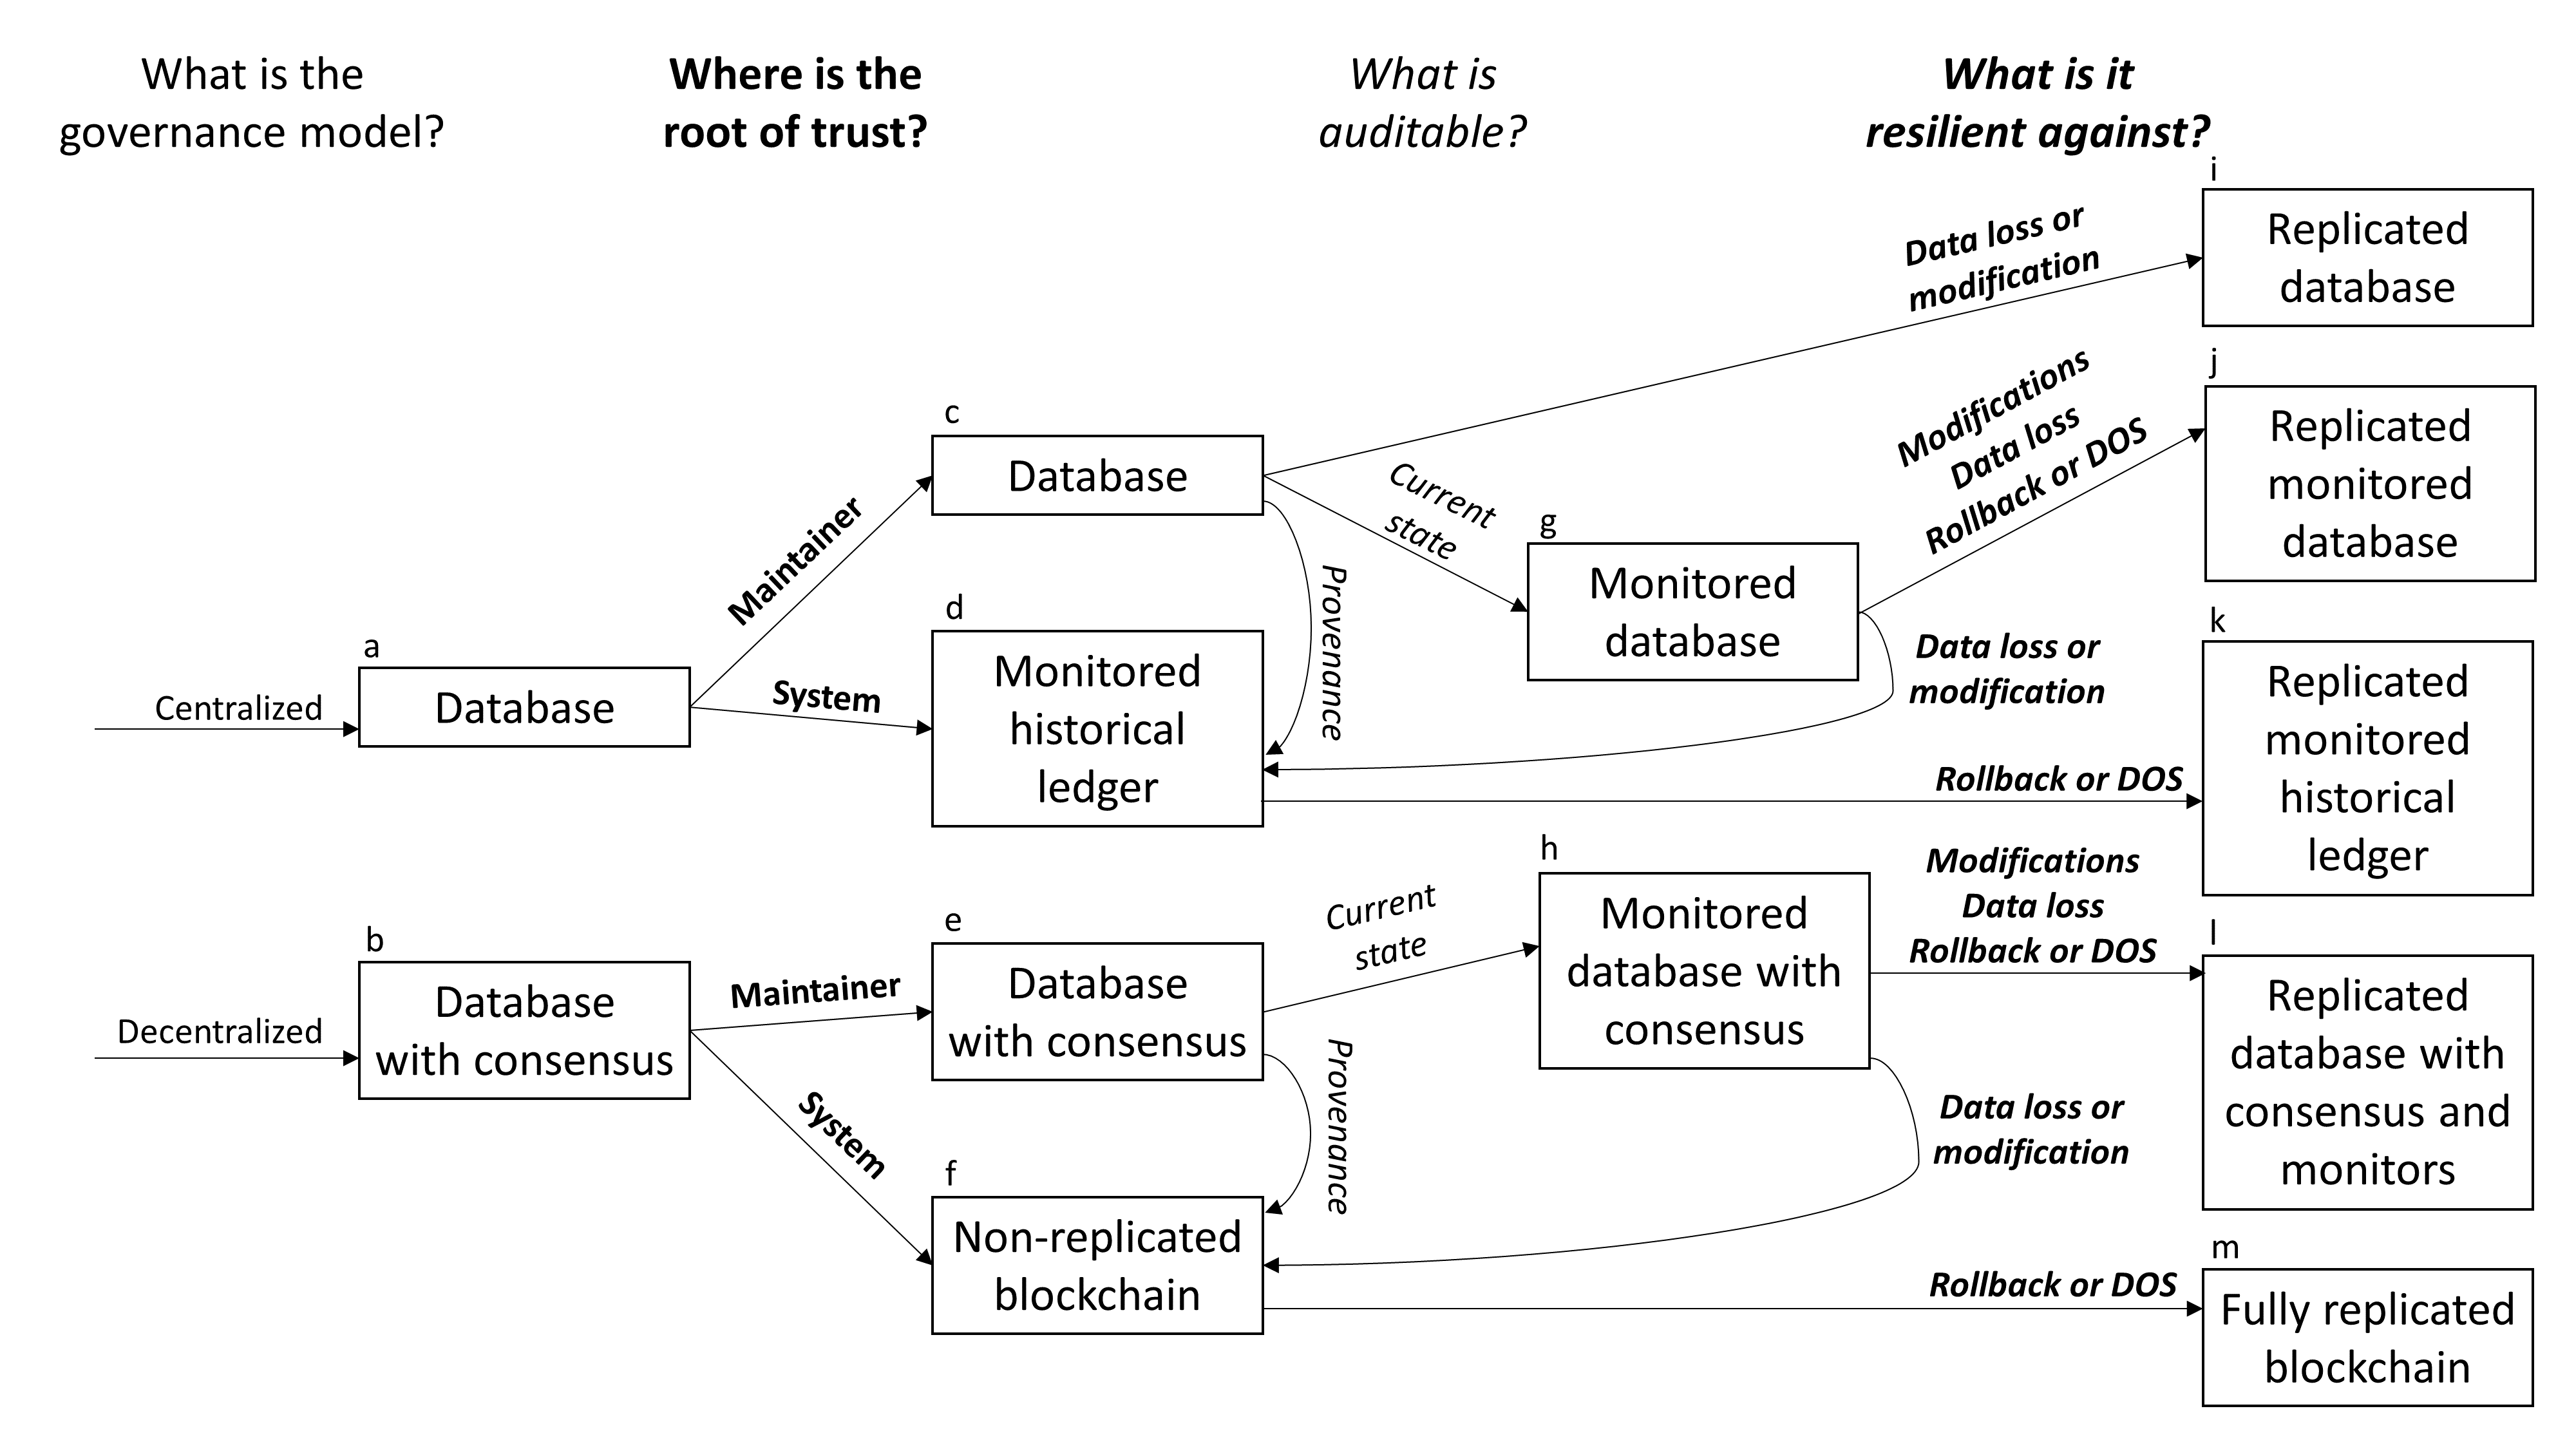
\includegraphics[width=\textwidth]{figures/BlockchainFlowchart.png}
	\caption{A classification of different database systems to illustrate Blockchain's place in the taxonomy}
	\label{fig:blockchainFlowchart}
\end{figure*}

The first question is about who has the authority to manage and update the database: \emph{what is the governance model?} In a centrally governed database (a), a single entity performs these tasks. Alternatively, the system can use a consensus protocol such as Byzantine Agreement to allow for decentralized governance (b).

Next, we consider the security model by asking \emph{where is the root of trust?} This refers to the entity or entities that must behave honestly in order for the system to be secure. In database systems, trust can either be rooted in the maintainer (e.g., a cloud storage provider) or it can be built into the design of the system itself (e.g., allowing user audits to ensure correct operation). For a centralized database to avoid trusting a maintainer, it must be possible for observers to verifiably reconstruct the current state of the data from the historical records of changes. We refer to such a system as a monitored historical ledger (d). Alternatively, a decentralized data store with no trusted maintainer is a blockchain (f), albeit one that is centrally stored (i.e., not replicated). 

In order for a system to be its own root of trust, stored data must be auditable back to its origin. However, for databases that rely on trusted maintainers, there are two possible ways for data to be verified by observers, and the next question deals with this: \emph{what is auditable?} If a centralized database with a trusted maintainer permits auditing of the current state, it is a monitored database (g), a good example of which is Google's Certificate Transparency project~\cite{CT}. If the data can be verified back to its origin using provenance, it's a monitored historical ledger as defined previously. A decentralized database has the same two options: if only current state is auditable, the system is a monitored database with consensus (h), but if provenance is available so that data can be audited back to its origin, it is a blockchain (f).

Finally, a database can have resilience properties depending on its design, so we ask \emph{what is it resilient against?} To prevent or recover from data loss or unauthorized modification, data can be replicated across multiple storage locations. The simplest case is a replicated database (i), but if the system also permits monitoring, replication also provides resilience to state rollback. We call this a replicated monitored database (j).
\bnote{Need to discuss the last column of this figure with Scott. How does DoS fit in, and how does the back edge from (g) to (d) provide resilience to data loss if the data isn't replicated?}

\subsection{Challenges and limitations}
\label{subsec:challenges}

% Jeremy: I reclustered this a bit. I think we discussed this during the call. Feel free to debate. 
% If you want to play around with the clusters: https://drive.google.com/file/d/1gDVd4x-SN6-QHZe52toEzMWXnLfiNtqW/view?usp=sharing
% I feel like separating challenges and limitations is a bit of a judgement call. 

Our concept map shows interconnections between features and use cases. We also coded challenges -- both problems hindering the use of Blockchain that do not currently have satisfactory solutions, and inherent deficits of the technology. In this section, we will list the concept groupings we created and we discuss the academic response in the next section.
\anote{I really like this list.  But, the challenges in Section~\ref{sec:challenges} only cover a subset of the list (and its not divided in the same way).  Should we aim to cover all the challenges listed here (for many of them, I dont really know what to say)?  We should definitely get the two sections to match up better.}
\subsubsection{Technical Challenges}
\begin{itemize}
	\item{Blockchain can handle finite, countable, and unique resources only}
	\item{Blockchain is not a high performance system}
	\item{Lack of API access means auditors must run full nodes}
	\item{Interoperability: cryptocurrency fragmentation; existence of too many implementations; siloed solutions; standardization; risks to overlay assets if underlying assets are mishandled; interfaces with existing institutions and systems; user identification across systems; risks posed by sharing blockchain security through merged mining or anchoring}	
        \item{Susceptibility to coordinated attacks by large parties}
	\item{Off-chain functionality: off-chain program execution; interoperability with off-chain systems}
	\item{Privacy: anonymity; confidentiality}
	\item{Resilience: distributed denial-of-service (DDOS) attacks; dishonest majority attacks; security of infrastructure; subversion of software security measures}		
	\item{Scalability: block generation frequency; block size limits; computational cost of public blockchains; scalable and secure end-user software}
	\item{Security}
	\item{Smart contract correctness: inherent incompleteness of contracts; ensuring completeness; lack of tools for verification}
\end{itemize}

\subsubsection{Socio-Technical Challenges}
\begin{itemize}
	\item{Blockchain is an inefficient use of computing resources}
	\item{Cryptocurrency economics: illiquidity, price volatility, high initial adoption costs, currency conversion costs, and decreasing marginal returns for miners}
	\item{Incentives: correctly configuring game-theoretic incentive structures}
	\item{Key management: difficulty of manual key management; possible unrecoverable loss of private keys; attacks against wallets; bugs and glitches in wallets}	
	\item{Lack of protection against mistakes: transactions cannot be reversed; administrators cannot restore access if users are locked out}
	\item{Miner centralization}
	\item{Usability: difficulty of developing distributed apps; inherent complexity of technology; difficulty of access and use by consumers; education; onboarding users; difficulty of search; poor UX; lack of mobile and web clients}
\end{itemize}

\subsubsection{Challenges to Market Viability}
\begin{itemize}
	\item{Efficiency and cost: low or bottlenecked throughput; wasteful energy consumption; high transaction fees; latency induced by synchronous communication required by certain consensus protocols}
	\item{Expense of developing end-user applications for individual blockchains}
	\item{Usefulness: few demonstrable use cases; does not improve upon existing solutions in many domains being pursued}
	\item{Unnecessary: if a central party is required; if a trusted intermediary exists; if a small number of parties are involved in the system}
\end{itemize}

\subsubsection{Use Case Challenges}
\begin{itemize}
	\item{Binding digital entities to real-world entities: stapling tokens to assets; interoperating with existing systems (e.g., compatibility between cryptocurrencies and cash)}
	\item{Dispute resolution: difficulty recovering from errors or bugs; difficulty reversing fraudulent transactions; non-applicability to scenarios where a central broker is needed}
\end{itemize}

\subsubsection{Regulatory Challenges}
\begin{itemize}
	\item{Governance: resolution of conflicts requiring external intervention; incident response; rule updates require forks; transparency of software development}
	\item{No distinct legal framework}
	\item{Standardization}
	\item{Regulatory: anti-money laundering, know-your-customer; difficulty of monitoring; lack of regulation; legal considerations; taxation; exchange control and flow management; consumer protection}	
	\item{Cryptocurrencies are inherently Ponzi schemes}
	\item{Reputation: use for crime; associations with black markets; nebulous or illicit uses; terrorist financing}
\end{itemize}

\section{Lessons Learned (Scott/Ben)}

What was missing in the graph?
Off-chain stapling
Anonymity
MPC
Functional encryption
Authenticated data structure

Terminology

Normative vs. technical properties
public participation is a huge normative property. Not gauntleted to be in a Blockchain.
There are risks of thinking they are the same
Using blockchain assuming you get normative properties, not just technical properties
Get saturated on normative properties, ignore the technical properties
Diffused trust vs. trustfulness
Decentralization
Governance and communication are required to be decentralized
Disintermediation is normative, and may or may not be part of a Blockchain
There are always intermediaries. Decentralization limits their power.



How do we know which use cases are good fits for Blockchain?
Criteria
1) Decentralized governance (*)
2) Auditability
3) Resiliency	
Is there a question tree we can create?